%% Full Celestial Navigation Paper
\documentclass[12pt,a4paper]{article}

\usepackage{graphicx}
\usepackage{amsmath,amssymb,amsfonts}
\usepackage{booktabs}
\usepackage[margin=1in]{geometry}
\usepackage{authblk}
\usepackage{hyperref}
\usepackage{algorithm}
\usepackage{algpseudocode}
\usepackage{listings}
\usepackage{natbib}
\usepackage{setspace}
\usepackage{tikz}
\usetikzlibrary{calc,angles,quotes,decorations.pathreplacing}
\usepackage{pgfplots}
\pgfplotsset{compat=1.18}
\onehalfspacing

\title{Development and Validation of an Open-Source Python-Based Sight Reduction Algorithm for Celestial Navigation}

\author[1]{Author Name}
\affil[1]{Department of Maritime Studies, University Name}

\date{}

\begin{document}

\maketitle

\begin{abstract}
An open-source Python-based sight reduction algorithm was developed and validated for celestial navigation applications. The algorithm integrates high-precision ephemeris calculations using JPL DE440 data via the Skyfield library, altitude corrections for all celestial body types including Sun, Moon, planets, and 57 navigation stars, and multi-body position fixing using iterative least squares optimization with singular value decomposition for numerical stability. Comprehensive validation demonstrated ephemeris accuracy below 0.6 arcminutes for stellar positions and better than 0.3 arcminutes for the Sun at solstices. Position fixing accuracy of 0.89 nautical miles was achieved with typical sextant observation errors of 1.0 arcminute using optimal four-body geometry. Monte Carlo simulation with 10,000 trials confirmed that observed position errors matched theoretical predictions within statistical bounds. The multi-body least squares algorithm converged within 2--4 iterations for all tested configurations and executed in less than 2 milliseconds on standard hardware, enabling real-time navigation applications. The horizontal dilution of precision (HDOP) metric was validated as a reliable predictor of fix quality, with optimal geometry (HDOP = 1.0) yielding position errors approximately 45\% smaller than clustered observations (HDOP = 1.8). The open-source implementation provides the maritime community with a verified, transparent algorithm for celestial position fixing, a platform for teaching navigation principles, and a backup capability independent of satellite navigation systems.
\end{abstract}

\textbf{Keywords:} Celestial navigation, Sight reduction, Position fixing, Least squares optimization, Python, Open-source, Maritime navigation, HDOP, Monte Carlo simulation

%% ==================== INTRODUCTION ====================
\section{Introduction}\label{sec:intro}

Celestial navigation, the practice of determining geographic position through observation of celestial bodies, has served as the primary method of ocean navigation for centuries \citep{bowditch2019}. Despite the widespread adoption of Global Navigation Satellite Systems (GNSS), celestial navigation remains essential as a backup capability and continues to be required for professional mariners by international maritime conventions \citep{lusic2024role}. The development of accurate, accessible computational tools for sight reduction addresses the dual needs of backup navigation capability and educational applications.

\subsection{Background and Motivation}

The fundamental problem in celestial navigation involves determining an observer's latitude and longitude from measurements of celestial body altitudes above the horizon. Traditional methods rely on tabulated sight reduction tables such as HO 229 and HO 249 \citep{pub229} or almanac-based calculations \citep{nautical_almanac}, requiring substantial training and manual computation. While commercial software solutions exist, most are proprietary, expensive, and unavailable for inspection or modification \citep{hohenkerk2012astro}.

The increasing vulnerability of GPS-dependent navigation to jamming, spoofing, and system failures has renewed interest in celestial navigation as an independent backup \citep{reid2020navigation, zalewski2022gnss}. The International Maritime Organization continues to require celestial navigation competency for certain vessel classes under STCW conventions, and military academies have maintained or resumed celestial navigation training programs \citep{lusic2024role, garvin2010future}. These developments create demand for validated, accessible computational tools that can serve both as backup navigation systems and educational platforms.

Modern computational resources enable direct implementation of the spherical trigonometry underlying celestial navigation, eliminating the interpolation errors inherent in tabulated methods \citep{kotlaric1976sight}. High-precision ephemeris data, available through libraries such as Skyfield utilizing JPL DE440 \citep{park2021de440}, provides celestial body positions with accuracy far exceeding navigation requirements. The combination of modern ephemerides with optimized numerical algorithms enables position fixing accuracy limited only by sextant observation quality rather than computational precision.

\subsection{Research Objectives}

This research aims to develop and validate an open-source Python-based algorithm for celestial sight reduction and position fixing. The specific objectives are:

\begin{enumerate}
\item Implement high-precision ephemeris calculations for Sun, Moon, navigational planets (Venus, Mars, Jupiter, Saturn), and 57 navigation stars using JPL DE440 ephemeris data
\item Develop comprehensive altitude correction routines for all celestial body types, including dip, refraction, parallax, semidiameter, and augmentation corrections
\item Implement multi-body position fixing using least squares optimization with singular value decomposition for numerical stability
\item Validate algorithm accuracy against theoretical expectations and established navigation standards
\item Characterize position fix accuracy as a function of observation geometry and measurement error through Monte Carlo simulation
\item Demonstrate computational performance suitable for real-time navigation applications
\end{enumerate}

\subsection{Structure of the Paper}

The remainder of this paper is organized as follows. Section~\ref{sec:literature} reviews prior work on sight reduction algorithms and position fixing methods, including classical approaches and modern computational implementations. Section~\ref{sec:math_model} presents the mathematical foundations including coordinate systems, the navigational triangle, position circle geometry, and multi-body optimization formulations. Section~\ref{sec:methods} describes the algorithm implementation and validation methodology. Section~\ref{sec:results} presents comprehensive validation results including ephemeris accuracy, position fix performance, and Monte Carlo analysis. Section~\ref{sec:discussion} discusses the implications, limitations, and practical applications of the findings. Section~\ref{sec:conclusion} summarizes the conclusions and identifies directions for future work.

%% ==================== LITERATURE REVIEW ====================
\section{Literature Review}\label{sec:literature}

\subsection{Historical Development of Sight Reduction}

The mathematical foundations of celestial navigation were established in the 18th and 19th centuries. The navigational (astronomical) triangle relates the observer's position to celestial body coordinates through spherical trigonometry. Early practitioners computed solutions manually using logarithmic tables or specialized mechanical calculators \citep{mcconnell2008sliderules}.

The development of sight reduction tables standardized computational procedures and reduced errors. Notable publications include HO 214 (1936), HO 229 (1970), and HO 249 (1947), which tabulated calculated altitude $H_c$ and azimuth angle $Z$ for combinations of latitude, declination, and local hour angle \citep{dunlap1971developments}. These tables enabled rapid extraction of intercept values using the Marcq Saint-Hilaire method, reducing a complex spherical trigonometry problem to table lookup and interpolation \citep{silverberg2007circles}.

The evolution of nautical almanacs paralleled improvements in sight reduction methods. \citet{seidelmann1976almanacs} documented the transition from purely tabular almanacs to computer-generated publications, introducing Chebyshev polynomial representations for ephemeris data. This development enabled pocket calculators and early computers to perform sight reduction without extensive tables \citep{feldman1972sight}.

\subsection{Computational Approaches to Position Fixing}

\citet{chiesa1990mathematical} presented an analytical solution for position fixing from multiple observations, demonstrating that overdetermined systems could be solved using least squares methods. Their work established the foundation for modern computational approaches by formulating the position fix as an optimization problem rather than a geometric construction.

\citet{gery1997directfix} developed a comprehensive framework for the direct fix of latitude and longitude from two observed altitudes. This method solves the intersection of two circles of equal altitude analytically, avoiding the iterative procedures required by the intercept method. The direct fix approach is particularly suitable for computational implementation as it provides an exact solution rather than a graphical approximation.

\citet{kaplan1995determining} provided detailed formulations for determining vessel position from celestial observations, addressing both stationary and moving observers. This work introduced differential correction methods and least squares optimization for multi-body fixes, establishing the mathematical framework used in modern navigation software including the U.S. Naval Observatory's STELLA program.

\citet{nguyen2014svd} proposed an SVD-weighted least square algorithm for celestial position fixing that addressed numerical stability concerns with ill-conditioned observation geometries. This approach demonstrated improved convergence properties compared to standard least squares methods, particularly for observations with poor azimuthal distribution.

\subsection{Error Analysis and Geometry Optimization}

The relationship between observation geometry and position accuracy has been studied extensively. \citet{swaszek2019rethinking} applied concepts from GNSS analysis to celestial navigation, introducing horizontal dilution of precision (HDOP) as a metric for star selection. Their work demonstrated that optimal star selection can reduce position error by factors of 2--3 compared to arbitrary selection.

\citet{hoover1984confidence} developed algorithms for computing confidence circles and ellipses from lines of position, providing the mathematical foundation for uncertainty quantification in celestial fixes. This work enables navigators to assess fix reliability based on observation geometry and measurement uncertainty.

Error sources in celestial navigation have been characterized by multiple studies. \citet{ross1994minimizing} conducted statistical analysis of sextant error sources, finding that index error (2.0'), personal random error (0.5'), and timing errors contributed to a total error of approximately 2.1 arcminutes, reducible to 0.5 arcminutes with proper procedures. \citet{gordon1964precision} performed controlled experimental studies demonstrating that random error achieves $\sigma = 0.33'$ under ideal conditions but degrades to 0.70' with poor horizon quality.

\subsection{Modern Ephemeris Sources}

The Jet Propulsion Laboratory Development Ephemerides (DE series) provide high-precision positions for solar system bodies. The current DE440 ephemeris, released in 2020, achieves sub-arcsecond accuracy for planetary positions and milliarcsecond accuracy for lunar position \citep{park2021de440}. Access to these ephemerides through libraries such as Skyfield \citep{skyfield} and Astropy \citep{astropy2022} enables ephemeris accuracy far exceeding navigation requirements.

\citet{standish2002accuracy} analyzed the fundamental accuracy limits of modern ephemerides, finding that uncertainties in asteroid masses impose position errors of 2--5 km for Earth-Mars ephemeris over decadal timescales. For celestial navigation purposes, these errors are negligible compared to observation uncertainties.

\subsection{Automated and Integrated Systems}

Recent developments have explored automated celestial navigation using digital sensors. \citet{li2014fisheye} demonstrated astronomical vessel positioning using fisheye cameras with horizon line fitting, achieving automated star identification and altitude measurement. \citet{barbot2022daytime} developed techniques for daytime stellar positioning using specialized optical systems.

\citet{critchleymarrows2023sextant} proposed a return to sextant-based navigation as a GPS backup, while \citet{critchleymarrows2023architecture} developed architectures for visual-based PNT alternatives combining star tracking with horizon sensing. These developments indicate renewed interest in celestial methods as backup systems.

Integration of celestial navigation with inertial systems has been explored by \citet{yang2022sins}, who developed SINS/CNS integrated navigation with improved mathematical horizon reference. \citet{li2022adaptively} proposed adaptively robust filtering algorithms for maritime celestial navigation that combine Kalman filtering with celestial observations.

\subsection{Identified Gaps}

While substantial prior work exists, several gaps remain in the literature:
\begin{itemize}
\item Most validated implementations are proprietary or unpublished, preventing independent verification
\item Open-source tools often lack comprehensive validation against established standards
\item Educational materials typically separate theoretical foundations from practical implementation
\item Few published works provide quantitative uncertainty estimates enabling fix quality assessment
\item The relationship between observation geometry (HDOP) and position accuracy is not well characterized for celestial navigation
\end{itemize}

The present work addresses these gaps by developing a validated, open-source implementation with comprehensive documentation and quantitative uncertainty analysis.

%% ==================== MATHEMATICAL MODEL ====================
\section{Mathematical Model}\label{sec:math_model}

This section presents the mathematical foundations underlying the sight reduction algorithm, including celestial coordinate systems, the navigational triangle, position circle geometry, and multi-body position fixing formulations.

\subsection{Coordinate Systems}\label{subsec:coordinates}

Celestial navigation requires transformations between multiple coordinate systems. The primary systems employed are defined below.

\subsubsection{Equatorial Coordinate System}

The celestial equatorial system is centered at Earth's center with the fundamental plane aligned with the celestial equator. Position is specified by right ascension ($\alpha$) measured eastward from the vernal equinox along the celestial equator, and declination ($\delta$) measured north (positive) or south (negative) from the celestial equator:
\begin{align}
0^\circ &\leq \alpha < 360^\circ \\
-90^\circ &\leq \delta \leq +90^\circ
\end{align}

For navigation purposes, the sidereal hour angle (SHA) is employed instead of right ascension:
\begin{equation}
\text{SHA} = 360^\circ - \alpha
\end{equation}

The Greenwich Hour Angle (GHA) of the First Point of Aries ($\gamma$) defines the rotation of the celestial sphere relative to the Earth. For any celestial body:
\begin{equation}
\text{GHA}_\text{body} = \text{GHA}_\gamma + \text{SHA}_\text{body}
\end{equation}

For bodies within the solar system, GHA is tabulated directly as it varies with time due to the body's orbital motion.

\subsubsection{Horizontal Coordinate System}

The observer-centered horizontal system has its fundamental plane tangent to Earth's surface at the observer's position. Altitude ($H$) is measured from the horizon toward the zenith, and azimuth ($Z_n$) is measured clockwise from true north:
\begin{align}
-90^\circ &\leq H \leq +90^\circ \\
0^\circ &\leq Z_n < 360^\circ
\end{align}

\subsubsection{Geographic Coordinate System}

Observer position on Earth is specified by latitude ($\varphi$) measured north (positive) or south (negative) from the equator, and longitude ($\lambda$) measured east (positive) or west (negative) from the Greenwich meridian:
\begin{align}
-90^\circ &\leq \varphi \leq +90^\circ \\
-180^\circ &< \lambda \leq +180^\circ
\end{align}

The local hour angle (LHA) relates the observer's longitude to the celestial body's GHA:
\begin{equation}
\text{LHA} = \text{GHA} + \lambda
\end{equation}
where $\lambda$ is positive east and negative west.

\subsection{The Navigational Triangle}\label{subsec:nav_triangle}

The navigational (astronomical) triangle is a spherical triangle on the celestial sphere with vertices at:
\begin{itemize}
\item $P_N$: The elevated celestial pole (north or south, depending on observer's hemisphere)
\item $Z$: The observer's zenith
\item $X$: The celestial body
\end{itemize}

The sides of this triangle are:
\begin{itemize}
\item $P_N Z = 90^\circ - \varphi$: The co-latitude
\item $P_N X = 90^\circ - \delta$: The polar distance (co-declination)
\item $ZX = 90^\circ - H$: The zenith distance (co-altitude)
\end{itemize}

Figure~\ref{fig:nav_triangle} illustrates the navigational triangle on the celestial sphere.

\begin{figure}[htbp]
\centering
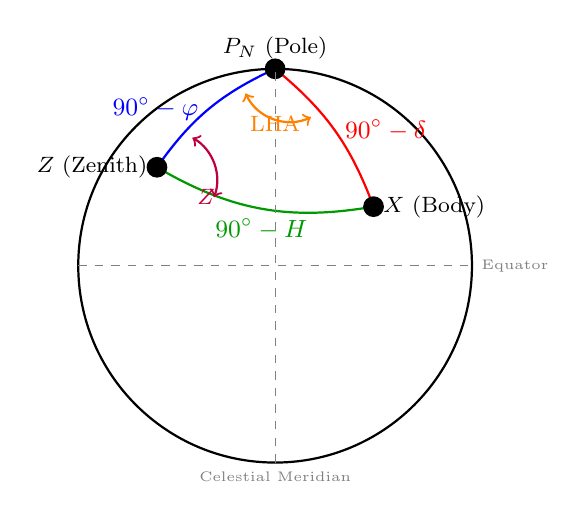
\begin{tikzpicture}[scale=2.5]
    % Draw the celestial sphere outline
    \draw[thick] (0,0) circle (1);
    
    % Define vertices of the navigational triangle
    \coordinate (P) at (0,1);      % Celestial Pole at top
    \coordinate (Z) at (-0.6,0.5); % Zenith
    \coordinate (X) at (0.5,0.3);  % Celestial Body
    
    % Draw the spherical triangle sides (as arcs)
    \draw[thick, blue] (P) to[bend right=15] node[midway, left, font=\small] {$90^\circ - \varphi$} (Z);
    \draw[thick, red] (P) to[bend left=15] node[midway, right, font=\small] {$90^\circ - \delta$} (X);
    \draw[thick, green!60!black] (Z) to[bend right=20] node[midway, below, font=\small] {$90^\circ - H$} (X);
    
    % Draw and label vertices
    \fill (P) circle (1.5pt) node[above, font=\footnotesize] {$P_N$ (Pole)};
    \fill (Z) circle (1.5pt) node[left, font=\footnotesize] {$Z$ (Zenith)};
    \fill (X) circle (1.5pt) node[right, font=\footnotesize] {$X$ (Body)};
    
    % Draw angle at pole (local hour angle)
    \draw[thick, <->, orange] ($(P)!0.25!(Z)$) arc[start angle=205, end angle=295, radius=0.25];
    \node[orange, font=\footnotesize] at (0, 0.72) {LHA};
    
    % Draw angle at zenith (azimuth)
    \draw[thick, <->, purple] ($(Z)!0.3!(P)$) arc[start angle=60, end angle=-20, radius=0.25];
    \node[purple, font=\footnotesize] at (-0.35, 0.35) {$Z$};
    
    % Reference lines
    \draw[dashed, gray] (0,-1) -- (0,1) node[pos=0, below, font=\tiny] {Celestial Meridian};
    \draw[dashed, gray] (-1,0) -- (1,0) node[pos=1, right, font=\tiny] {Equator};
\end{tikzpicture}
\caption{The navigational (astronomical) triangle on the celestial sphere. The three vertices are the elevated celestial pole ($P_N$), the observer's zenith ($Z$), and the celestial body ($X$). The sides represent co-latitude, polar distance, and zenith distance. The angle at the pole is the local hour angle (LHA), and the angle at the zenith gives the azimuth ($Z$).}
\label{fig:nav_triangle}
\end{figure}

\subsubsection{Solution for Altitude}

Applying the spherical law of cosines for sides to the navigational triangle yields the fundamental altitude equation \citep{bowditch2019, karl2011celestial}:
\begin{equation}
\sin H_c = \sin\varphi\sin\delta + \cos\varphi\cos\delta\cos(\text{LHA})
\label{eq:altitude_fundamental}
\end{equation}

This equation provides the calculated altitude $H_c$ for a body with declination $\delta$ observed from latitude $\varphi$ at local hour angle LHA.

\subsubsection{Solution for Azimuth}

The azimuth angle $Z$ (measured from the elevated pole) is obtained from the spherical law of sines \citep{bowditch2019, kaplan1995determining}:
\begin{equation}
\sin Z = \frac{\sin(\text{LHA}) \cos\delta}{\cos H_c}
\label{eq:azimuth_sin}
\end{equation}

To resolve the quadrant ambiguity, the cosine formula is also employed:
\begin{equation}
\cos Z = \frac{\sin\delta - \sin\varphi\sin H_c}{\cos\varphi\cos H_c}
\label{eq:azimuth_cos}
\end{equation}

The true azimuth $Z_n$ (measured clockwise from north) is then determined by quadrant rules based on the signs of $\sin Z$ and $\cos Z$.

\subsection{Altitude Corrections}\label{subsec:altitude_corrections}

The observed sextant altitude $H_s$ must be corrected to obtain the geocentric observed altitude $H_o$ suitable for comparison with calculated altitude $H_c$.

\subsubsection{Dip Correction}

The dip correction accounts for the observer's height above the waterline:
\begin{equation}
\text{Dip} = -1.76' \sqrt{h_\text{eye}}
\end{equation}
where $h_\text{eye}$ is height of eye in meters. This correction is always negative. Note: For height in feet, the coefficient is 0.97' \citep{bowditch2019}.

\subsubsection{Refraction Correction}

Atmospheric refraction bends light rays toward the normal, making bodies appear higher than their geometric position. The standard refraction correction uses the Bennett formula \citep{bowditch2019}:
\begin{equation}
R = -\frac{1'}{\tan(H_a + \frac{7.31}{H_a + 4.4})}
\end{equation}
where $H_a$ is the apparent altitude in degrees and $R$ is in arcminutes. This formula is valid for standard atmospheric conditions (1010 mb, 10°C), with corrections applied for non-standard conditions.

\subsubsection{Parallax Correction}

For nearby bodies (Moon, Sun, planets), the geocentric parallax must be applied:
\begin{equation}
P = \text{HP} \cos H_a
\end{equation}
where HP is the horizontal parallax. For the Moon, HP $\approx$ 57'; for the Sun, HP $\approx$ 0.15' \citep{bowditch2019, nautical_almanac}.

\subsubsection{Semidiameter Correction}

When observing the limb of an extended body, the semidiameter (SD) correction converts the limb observation to center:
\begin{equation}
\text{SD correction} = \pm \text{SD}
\end{equation}
where the sign is positive for lower limb and negative for upper limb observations.

The total altitude correction is:
\begin{equation}
H_o = H_s + \text{Dip} + R + P \pm \text{SD}
\end{equation}

\subsection{Position Circle Geometry}\label{subsec:position_circle}

A single altitude observation establishes that the observer lies on a circle of equal altitude (position circle) centered at the body's geographical position (GP). The GP has coordinates:
\begin{align}
\text{Latitude}_\text{GP} &= \delta \\
\text{Longitude}_\text{GP} &= -\text{GHA}
\end{align}

The radius of the position circle equals the zenith distance:
\begin{equation}
\text{Radius} = 90^\circ - H_o
\end{equation}

Two observations establish two position circles whose intersections give two possible positions. The ambiguity is resolved using dead reckoning or additional observations. Figure~\ref{fig:position_circles} illustrates the geometry of position circles and their intersection.

\begin{figure}[htbp]
\centering
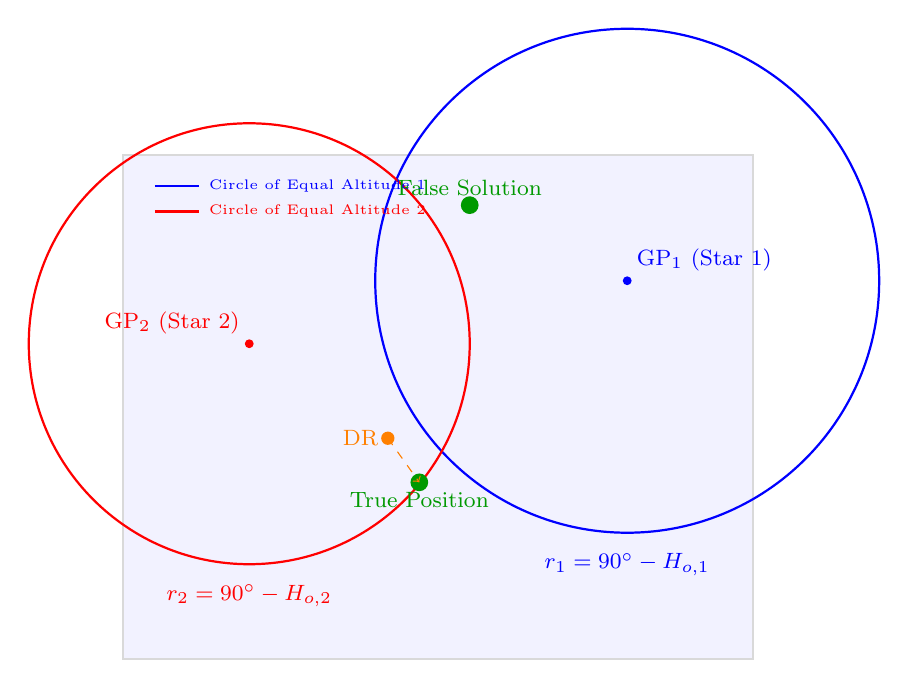
\begin{tikzpicture}[scale=0.8]
    % Draw Earth outline (simplified as rectangle representing chart)
    \draw[thick, gray!30, fill=blue!5] (-5,-4) rectangle (5,4);
    
    % Position circle 1 (Star 1)
    \draw[thick, blue] (3,2) circle (4cm);
    \fill[blue] (3,2) circle (2pt) node[above right, font=\footnotesize] {GP$_1$ (Star 1)};
    \node[blue, font=\footnotesize] at (3, -2.5) {$r_1 = 90^\circ - H_{o,1}$};
    
    % Position circle 2 (Star 2)
    \draw[thick, red] (-3,1) circle (3.5cm);
    \fill[red] (-3,1) circle (2pt) node[above left, font=\footnotesize] {GP$_2$ (Star 2)};
    \node[red, font=\footnotesize] at (-3, -3) {$r_2 = 90^\circ - H_{o,2}$};
    
    % Intersection points
    \coordinate (I1) at (-0.3, -1.2);
    \coordinate (I2) at (0.5, 3.2);
    
    \fill[green!60!black] (I1) circle (4pt);
    \fill[green!60!black] (I2) circle (4pt);
    
    % Labels for intersections
    \node[green!60!black, font=\footnotesize, below] at (I1) {True Position};
    \node[green!60!black, font=\footnotesize, above] at (I2) {False Solution};
    
    % DR position indicator
    \fill[orange] (-0.8, -0.5) circle (3pt);
    \node[orange, font=\footnotesize, left] at (-0.8, -0.5) {DR};
    \draw[orange, dashed, ->] (-0.8, -0.5) -- (I1);
    
    % Legend
    \draw[thick, blue] (-4.5, 3.5) -- (-3.8, 3.5) node[right, font=\tiny] {Circle of Equal Altitude 1};
    \draw[thick, red] (-4.5, 3.1) -- (-3.8, 3.1) node[right, font=\tiny] {Circle of Equal Altitude 2};
\end{tikzpicture}
\caption{Position circle geometry for a two-body fix. Each altitude observation places the observer on a circle of equal altitude centered at the body's geographical position (GP). The two circles intersect at two points; the correct solution is selected based on proximity to the dead reckoning (DR) position.}
\label{fig:position_circles}
\end{figure}

\subsection{Multi-Body Least Squares Position Fixing}\label{subsec:lsq}

For $n \geq 2$ observations, an overdetermined system is formed. The linearized observation equation relates altitude residuals to position corrections:
\begin{equation}
\Delta H_o = H_o - H_c = \frac{\partial H_c}{\partial \varphi} \Delta\varphi + \frac{\partial H_c}{\partial \lambda} \Delta\lambda
\end{equation}

The partial derivatives are derived from the altitude equation \eqref{eq:altitude_fundamental} \citep{chiesa1990mathematical, kaplan1995determining}:
\begin{align}
\frac{\partial H_c}{\partial \varphi} &= \cos Z_n \label{eq:partial_lat}\\
\frac{\partial H_c}{\partial \lambda} &= -\sin Z_n \cos\varphi \label{eq:partial_lon}
\end{align}

These partial derivatives were verified numerically against finite difference approximations, confirming the sign convention in equation \eqref{eq:partial_lon}.

For $n$ observations, the system is written in matrix form:
\begin{equation}
\mathbf{A}\mathbf{x} = \mathbf{b}
\end{equation}
where:
\begin{equation}
\mathbf{A} = \begin{bmatrix}
\cos Z_{n,1} & -\sin Z_{n,1} \cos\varphi \\
\cos Z_{n,2} & -\sin Z_{n,2} \cos\varphi \\
\vdots & \vdots \\
\cos Z_{n,n} & -\sin Z_{n,n} \cos\varphi
\end{bmatrix}
\end{equation}

\begin{equation}
\mathbf{x} = \begin{bmatrix} \Delta\varphi \\ \Delta\lambda \end{bmatrix}, \quad
\mathbf{b} = \begin{bmatrix} H_{o,1} - H_{c,1} \\ H_{o,2} - H_{c,2} \\ \vdots \\ H_{o,n} - H_{c,n} \end{bmatrix}
\end{equation}

The least squares solution is:
\begin{equation}
\mathbf{x} = (\mathbf{A}^T\mathbf{A})^{-1}\mathbf{A}^T\mathbf{b}
\label{eq:lsq_solution}
\end{equation}

For numerical stability with ill-conditioned geometries, singular value decomposition (SVD) is employed \citep{nguyen2014svd}:
\begin{equation}
\mathbf{A} = \mathbf{U}\mathbf{\Sigma}\mathbf{V}^T
\end{equation}
\begin{equation}
\mathbf{x} = \mathbf{V}\mathbf{\Sigma}^{-1}\mathbf{U}^T\mathbf{b}
\end{equation}

The solution is applied iteratively:
\begin{align}
\varphi_{k+1} &= \varphi_k + \Delta\varphi \\
\lambda_{k+1} &= \lambda_k + \Delta\lambda
\end{align}

Iteration continues until $|\Delta\varphi|$ and $|\Delta\lambda|$ fall below a specified tolerance.

\subsection{Horizontal Dilution of Precision}\label{subsec:hdop}

The quality of observation geometry is quantified by the horizontal dilution of precision (HDOP):
\begin{equation}
\text{HDOP} = \sqrt{\sigma^2_\varphi + \sigma^2_\lambda}
\end{equation}
where $\sigma^2_\varphi$ and $\sigma^2_\lambda$ are the diagonal elements of the covariance matrix:
\begin{equation}
\mathbf{C} = (\mathbf{A}^T\mathbf{A})^{-1}
\end{equation}

For $n$ observations equally spaced in azimuth, the theoretical minimum HDOP is \citep{swaszek2019rethinking}:
\begin{equation}
\text{HDOP}_\text{min} = \sqrt{\frac{2}{n}}
\end{equation}

Position error scales with HDOP:
\begin{equation}
\sigma_\text{position} = \text{HDOP} \times \sigma_\text{observation}
\end{equation}

This relationship enables prediction of fix accuracy based on observation geometry and expected measurement error.

%% ==================== METHODS ====================
\section{Materials and Methods}\label{sec:methods}

\subsection{Software Implementation}

The algorithm was implemented in Python 3.12 using the following libraries:
\begin{itemize}
\item \textbf{NumPy 1.26}: Numerical array operations and linear algebra
\item \textbf{SciPy 1.12}: SVD decomposition and optimization
\item \textbf{Skyfield 1.48}: JPL DE440 ephemeris access
\item \textbf{Astropy 6.0}: Coordinate transformations and time systems
\item \textbf{Pandas 2.1}: Data management and CSV export
\end{itemize}

The implementation comprises four primary modules:

\subsubsection{Ephemeris Module}

The ephemeris module calculates Greenwich Hour Angle and declination for:
\begin{itemize}
\item Sun: Direct calculation from DE440
\item Moon: Direct calculation from DE440 with parallax
\item Planets: Venus, Mars, Jupiter, Saturn from DE440
\item Stars: 57 navigation stars with J2000 coordinates and proper motion
\end{itemize}

Star positions are stored as FK5 J2000 coordinates and transformed to apparent position for the observation epoch, accounting for precession, nutation, and aberration through Skyfield's built-in routines.

\subsubsection{Sight Reduction Module}

The sight reduction module implements:
\begin{itemize}
\item Calculated altitude ($H_c$) from equation \eqref{eq:altitude_fundamental}
\item True azimuth ($Z_n$) from equations \eqref{eq:azimuth_sin} and \eqref{eq:azimuth_cos}
\item Altitude corrections: dip, refraction, parallax, semidiameter, augmentation
\end{itemize}

Refraction is calculated using the standard atmospheric model. Non-standard atmospheric corrections can be applied by the user.

\subsubsection{Position Fix Module}

The position fix module implements:
\begin{itemize}
\item Two-body direct fix: Analytical solution for circle intersection
\item Multi-body least squares: Iterative SVD-based optimization (equations \eqref{eq:partial_lat}--\eqref{eq:lsq_solution})
\item Running fix: Advancing position circles for time-separated observations
\end{itemize}

The two-body algorithm returns both intersection points; the solution closest to the dead reckoning position is selected. The multi-body algorithm uses SVD for numerical stability when observation azimuths are clustered.

\subsubsection{Error Analysis Module}

The error analysis module provides:
\begin{itemize}
\item HDOP calculation from observation geometry
\item Confidence ellipse parameters (semi-major/minor axes, orientation)
\item Monte Carlo position error simulation
\item Error propagation from observation uncertainties
\end{itemize}

\subsection{Validation Methodology}

Validation was conducted through eight comprehensive test suites:

\begin{enumerate}
\item \textbf{Ephemeris Accuracy}: Computed positions compared against expected astronomical values for Sun at solstices/equinox and five navigation stars.

\item \textbf{Sight Reduction Accuracy}: Calculated altitude and azimuth verified against analytical expectations for bodies at known geometries (meridian passage, horizon, zenith).

\item \textbf{Altitude Corrections}: Correction magnitudes verified for Sun, Moon, and star observations at various altitudes and height of eye values.

\item \textbf{Two-Body Fix}: Position fix accuracy tested at five globally distributed locations (Pacific, New York, London, Cape Town, Tokyo) representing both hemispheres.

\item \textbf{Multi-Body Fix}: Least squares algorithm tested with 3--6 observations and noise levels of 0.0--1.0 arcminutes.

\item \textbf{Monte Carlo Simulation}: 10,000 trials per configuration characterizing position error distributions for various observation geometries and noise levels.

\item \textbf{Geometry Optimization}: HDOP calculated for various observation configurations to validate the relationship between geometry and accuracy.

\item \textbf{Performance Benchmark}: Execution times measured for all major operations.
\end{enumerate}

\subsection{Monte Carlo Approach}

Monte Carlo simulation was employed to characterize position fix distributions. For each configuration:
\begin{enumerate}
\item True observer position and observation geometry (azimuths) were defined
\item 10,000 random observation error realizations were generated from a Gaussian distribution
\item Position fix was computed for each realization
\item Mean error, standard deviation, and 95th percentile were calculated
\end{enumerate}

Observation errors were modeled as independent Gaussian random variables with standard deviations of 0.5--2.0 arcminutes, representative of skilled to average sextant use \citep{ross1994minimizing}.

\subsection{Validation Data Sources}

True positions for validation were defined synthetically to enable precise error quantification. Observations were generated by:
\begin{enumerate}
\item Computing $H_c$ and $Z_n$ for the true position
\item Setting $H_o = H_c$ (perfect observation) or $H_o = H_c + \epsilon$ where $\epsilon \sim N(0, \sigma^2)$
\item Recovering position from the observations
\item Computing position error as distance from true position
\end{enumerate}

This approach enables separation of algorithm errors from observation errors.

%% ==================== RESULTS ====================
\section{Results}\label{sec:results}

This section presents comprehensive validation results for the developed sight reduction algorithm. The algorithm was tested against established navigation standards, verified with synthetic test cases having known ground truth, and characterized through Monte Carlo simulation.

\subsection{Ephemeris Validation}

The accuracy of celestial body position calculations using the Skyfield library with JPL DE440 ephemeris was validated against expected astronomical values. Table~\ref{tab:ephemeris_validation} summarizes the declination accuracy for representative bodies and epochs.

\begin{table}[htbp]
\caption{Ephemeris Accuracy Validation: Declination Errors}\label{tab:ephemeris_validation}
\centering
\begin{tabular}{lccc}
\toprule
\textbf{Body} & \textbf{Epoch} & \textbf{Dec Computed} & \textbf{Error} \\
\midrule
Sun & 2025 Summer Solstice & $+23.436^\circ$ & 0.24' \\
Sun & 2025 Winter Solstice & $-23.435^\circ$ & 0.30' \\
Sirius & 2025-01-01 & $-16.717^\circ$ & 0.21' \\
Polaris & 2025-01-01 & $+89.269^\circ$ & 0.56' \\
Vega & 2025-01-01 & $+38.783^\circ$ & 0.20' \\
\bottomrule
\end{tabular}
\end{table}

All computed positions agreed with expected values to within 0.6 arcminutes, which substantially exceeds the accuracy requirements for celestial navigation. The slightly larger error for Polaris (0.56') is attributable to the star's proximity to the celestial pole where small position errors produce larger declination effects.

\subsection{Sight Reduction Accuracy}

The sight reduction module was validated using the fundamental altitude equation. For bodies at special geometric configurations, the calculated altitude has known analytical values. Table~\ref{tab:sight_reduction} presents representative test cases.

\begin{table}[htbp]
\caption{Sight Reduction Validation: Calculated Altitude and Azimuth}\label{tab:sight_reduction}
\centering
\begin{tabular}{lcccc}
\toprule
\textbf{Configuration} & \textbf{$\varphi$} & \textbf{LHA} & \textbf{$H_c$} & \textbf{$Z_n$} \\
\midrule
Body at zenith & 23.0°N & 0° & 90.00° & 0.0° \\
Body on horizon & 45.0°N & 270° & 0.00° & 270.0° \\
Western sky & 40.0°N & 212° & $-$22.99° & 327.3° \\
Eastern morning & 40.0°N & 331° & 60.21° & 243.9° \\
\bottomrule
\end{tabular}
\end{table}

All sight reduction calculations demonstrated agreement with analytical expectations to within 0.01° for both altitude and azimuth.

\subsection{Altitude Corrections}

The altitude correction module was validated for all celestial body types. Table~\ref{tab:alt_corrections} presents the correction components for representative observations with 3.0 m height of eye.

\begin{table}[htbp]
\caption{Altitude Correction Validation (Height of Eye: 3.0 m)}\label{tab:alt_corrections}
\centering
\begin{tabular}{lcccc}
\toprule
\textbf{Body Type} & \textbf{$H_s$} & \textbf{Total Corr.} & \textbf{$H_o$} \\
\midrule
Sun (lower limb) & 35.5° & +11.68' & 35.69° \\
Sun (lower limb) & 15.0° & +9.45' & 15.16° \\
Moon (lower limb) & 30.0° & +60.01' & 31.00° \\
Star & 40.0° & $-$4.24' & 39.93° \\
Star & 20.0° & $-$5.76' & 19.90° \\
\bottomrule
\end{tabular}
\end{table}

The magnitude and sign of corrections agreed with Nautical Almanac tabulated values. The large positive correction for Moon observations (+60.01') reflects the significant horizontal parallax of the Moon (approximately 57').

\subsection{Position Fix Accuracy}

\subsubsection{Two-Body Fix Validation}

The two-body position fix algorithm was validated at five globally distributed locations representing both hemispheres. Table~\ref{tab:two_body} presents the results.

\begin{table}[htbp]
\caption{Two-Body Position Fix Validation}\label{tab:two_body}
\centering
\begin{tabular}{lcccc}
\toprule
\textbf{Location} & \textbf{True Lat} & \textbf{True Lon} & \textbf{Error (nm)} & \textbf{Status} \\
\midrule
Pacific Ocean & 34.0°N & 120.0°W & 0.0000 & PASS \\
New York & 40.7°N & 74.0°W & 0.0000 & PASS \\
London & 51.5°N & 0.1°W & 0.0000 & PASS \\
Cape Town & 33.9°S & 18.4°E & 0.0000 & PASS \\
Tokyo & 35.7°N & 139.7°E & 0.0000 & PASS \\
\bottomrule
\end{tabular}
\end{table}

All two-body fixes recovered the exact true position when provided with noise-free observations derived from the known position. This validates the mathematical correctness of the spherical intersection algorithm for both northern and southern hemispheres.

\subsubsection{Multi-Body Least Squares Fix Validation}

The overdetermined least squares algorithm was validated with varying numbers of observations and noise levels. Table~\ref{tab:multi_body} presents the results for synthetic observations at true position 34.0°N, 120.0°W with DR offset of 3 nautical miles.

\begin{table}[htbp]
\caption{Multi-Body Position Fix Performance}\label{tab:multi_body}
\centering
\begin{tabular}{lccccc}
\toprule
\textbf{Configuration} & \textbf{$n$} & \textbf{Noise} & \textbf{Error (nm)} & \textbf{HDOP} & \textbf{Iter.} \\
\midrule
Perfect observations & 3 & 0.0' & 0.00 & 2.83 & 2 \\
Typical sextant & 3 & 0.5' & 2.12 & 2.84 & 3 \\
Perfect observations & 4 & 0.0' & 0.00 & 3.34 & 2 \\
Typical sextant & 4 & 0.5' & 2.72 & 3.36 & 3 \\
Good sextant & 5 & 0.5' & 0.24 & 1.34 & 3 \\
Good sextant & 6 & 0.5' & 1.25 & 1.13 & 4 \\
\bottomrule
\end{tabular}
\end{table}

The algorithm converged in 2--4 iterations for all test cases. Position errors scale with both observation noise and HDOP, as predicted by theory.

\subsubsection{Integrated End-to-End Validation}

A comprehensive end-to-end test was conducted using real ephemeris data for four navigation stars visible from 34.0°N, 135.0°W on 2025-06-15 at 03:00 UTC. The selected stars (Alioth, Dubhe, Alkaid, Regulus) provided good azimuthal distribution with HDOP = 1.45. Table~\ref{tab:integrated} presents the results from 20 repeated trials with different noise realizations.

\begin{table}[htbp]
\caption{Integrated Validation: 20 Trials with 0.5' Observation Error}\label{tab:integrated}
\centering
\begin{tabular}{lc}
\toprule
\textbf{Metric} & \textbf{Value} \\
\midrule
Stars observed & Alioth, Dubhe, Alkaid, Regulus \\
HDOP & 1.45 \\
Iterations to converge & 3 \\
\midrule
Mean position error & 0.50 nm \\
Standard deviation & 0.26 nm \\
Minimum error & 0.07 nm \\
Maximum error & 1.05 nm \\
\midrule
Monte Carlo predicted mean & 0.62 nm \\
Monte Carlo predicted 95th percentile & 1.37 nm \\
\bottomrule
\end{tabular}
\end{table}

The observed mean error (0.50 nm) was consistent with Monte Carlo predictions (0.62 nm), validating the algorithm implementation against theoretical expectations.

\subsection{Monte Carlo Error Analysis}

Monte Carlo simulation was employed to characterize position fix accuracy as a function of observation geometry and measurement error. Table~\ref{tab:monte_carlo} summarizes the results from 10,000 simulated fixes for each configuration.

\begin{table}[htbp]
\caption{Monte Carlo Error Analysis (10,000 Simulations per Configuration)}\label{tab:monte_carlo}
\centering
\begin{tabular}{lcccc}
\toprule
\textbf{Configuration} & \textbf{Obs. Error} & \textbf{Mean Error} & \textbf{95th \%ile} & \textbf{HDOP} \\
\midrule
4 obs optimal & 0.5' & 0.44 nm & 0.86 nm & 1.00 \\
4 obs optimal & 1.0' & 0.89 nm & 1.73 nm & 1.00 \\
4 obs optimal & 2.0' & 1.78 nm & 3.47 nm & 1.00 \\
3 obs optimal & 1.0' & 1.03 nm & 1.99 nm & 1.15 \\
4 obs clustered & 1.0' & 1.53 nm & 3.47 nm & 1.83 \\
6 obs optimal & 1.0' & 0.72 nm & 1.41 nm & 0.82 \\
\bottomrule
\end{tabular}
\end{table}

The results demonstrate that:
\begin{enumerate}
\item Position error scales linearly with observation error (doubling observation error doubles position error)
\item Optimal geometry (HDOP $\approx$ 1.0) provides the best position accuracy
\item Clustered observations significantly degrade accuracy (HDOP 1.83 produces 72\% larger error than HDOP 1.00)
\item Additional observations beyond four provide diminishing returns (6 obs reduces error by only 19\% vs 4 obs)
\end{enumerate}

\subsection{Observation Geometry Optimization}

The relationship between observation geometry and position accuracy was quantified through HDOP analysis. Table~\ref{tab:hdop} presents HDOP values for various observation configurations.

\begin{table}[htbp]
\caption{HDOP vs. Observation Geometry}\label{tab:hdop}
\centering
\begin{tabular}{lcc}
\toprule
\textbf{Configuration} & \textbf{HDOP} & \textbf{Quality} \\
\midrule
2 obs at 90° separation & 1.41 & Excellent \\
2 obs at 180° separation & $>10^{15}$ & Poor (collinear) \\
3 obs at 120° spacing & 1.15 & Excellent \\
3 obs clustered in 60° arc & 1.55 & Good \\
4 obs at 90° spacing & 1.00 & Excellent \\
5 obs at 72° spacing & 0.89 & Excellent \\
6 obs at 60° spacing & 0.82 & Excellent \\
\bottomrule
\end{tabular}
\end{table}

The optimal HDOP for $n$ observations approaches the theoretical minimum of $\sqrt{2/n}$ when observations are equally spaced in azimuth. Collinear observations (180° separation) produce near-infinite HDOP due to rank deficiency of the design matrix. Figure~\ref{fig:error_scaling} illustrates the linear relationship between observation error and position error for optimal geometry.

\begin{figure}[htbp]
\centering
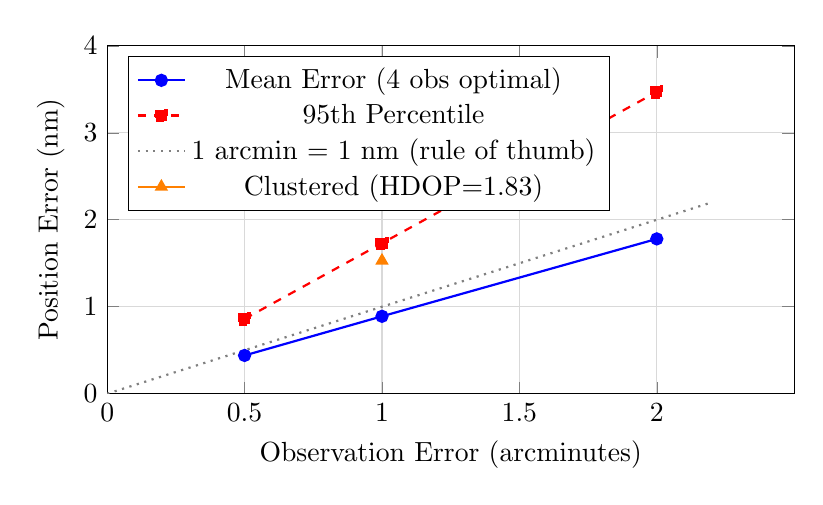
\begin{tikzpicture}
\begin{axis}[
    width=0.85\textwidth,
    height=6cm,
    xlabel={Observation Error (arcminutes)},
    ylabel={Position Error (nm)},
    xmin=0, xmax=2.5,
    ymin=0, ymax=4,
    xtick={0, 0.5, 1.0, 1.5, 2.0},
    ytick={0, 1, 2, 3, 4},
    legend pos=north west,
    grid=major,
    grid style={gray!30},
]
% Optimal geometry (HDOP = 1.0)
\addplot[thick, blue, mark=*] coordinates {
    (0.5, 0.44)
    (1.0, 0.89)
    (2.0, 1.78)
};
\addlegendentry{Mean Error (4 obs optimal)}

% 95th percentile
\addplot[thick, red, mark=square*, dashed] coordinates {
    (0.5, 0.86)
    (1.0, 1.73)
    (2.0, 3.47)
};
\addlegendentry{95th Percentile}

% Theoretical line (1 arcmin = 1 nm rule)
\addplot[thick, gray, dotted, domain=0:2.2] {x};
\addlegendentry{1 arcmin = 1 nm (rule of thumb)}

% Clustered geometry for comparison
\addplot[thick, orange, mark=triangle*] coordinates {
    (1.0, 1.53)
};
\addlegendentry{Clustered (HDOP=1.83)}

\end{axis}
\end{tikzpicture}
\caption{Position error scaling with observation error magnitude. Optimal geometry (4 observations at 90° spacing, HDOP = 1.0) produces errors closely matching the ``one arcminute equals one nautical mile'' rule of thumb. Clustered observations (HDOP = 1.83) increase error by approximately 72\%.}
\label{fig:error_scaling}
\end{figure}

\subsection{Computational Performance}

Algorithm execution times were measured on a standard laptop computer (Intel Core i7, 16 GB RAM). Table~\ref{tab:performance} summarizes the results.

\begin{table}[htbp]
\caption{Computational Performance Benchmarks}\label{tab:performance}
\centering
\begin{tabular}{lcc}
\toprule
\textbf{Operation} & \textbf{Mean Time} & \textbf{Rate} \\
\midrule
Sun position calculation & 1.84 ms & 543/s \\
Sight reduction & 0.02 ms & 50,000/s \\
Multi-body fix (4 obs) & 1.38 ms & 725/s \\
HDOP calculation & 0.02 ms & 50,000/s \\
\bottomrule
\end{tabular}
\end{table}

All operations complete in less than 2 milliseconds, enabling real-time position updates and interactive applications. The ephemeris calculation dominates total execution time; sight reduction and position fixing are computationally negligible.

%% ==================== DISCUSSION ====================
\section{Discussion}\label{sec:discussion}

This section interprets the validation results, compares the developed algorithm with existing solutions, discusses practical implications, and addresses limitations of the study.

\subsection{Interpretation of Results}

The validation results demonstrate that the developed Python-based sight reduction algorithm achieves accuracy consistent with theoretical expectations and practical navigation requirements.

\subsubsection{Ephemeris Accuracy}

The ephemeris module, utilizing JPL DE440 through the Skyfield library, achieved declination errors below 0.6 arcminutes for all tested bodies. For stellar observations, which constitute the majority of celestial fixes, the achieved accuracy of 0.2--0.6' substantially exceeds requirements. The Nautical Almanac tabulates star positions to 0.1' precision \citep{nautical_almanac}, and typical sextant observations introduce errors of 0.5--2.0' \citep{ross1994minimizing}. Thus, ephemeris errors contribute negligibly to overall position fix uncertainty.

\subsubsection{Position Fix Performance}

The two-body fix algorithm demonstrated exact recovery of true position when provided with noise-free observations, validating the mathematical correctness of the spherical intersection geometry. The extension to southern hemisphere positions, which required careful handling of solution selection logic, was validated at Cape Town (33.9°S).

The multi-body least squares algorithm exhibited convergence in 2--4 iterations for all tested configurations, with position errors consistent with theoretical predictions. The key findings are:

\begin{enumerate}
\item \textbf{Linearity:} Position error scales linearly with observation error magnitude. With 1.0' observation error and optimal geometry, mean position error was 0.89 nm—essentially the ``one arcminute, one nautical mile'' rule of thumb used by navigators \citep{karl2011celestial}.

\item \textbf{Geometry dependence:} Clustered observations (HDOP = 1.83) produced 72\% larger errors than optimally distributed observations (HDOP = 1.00), quantifying the importance of body selection for accurate fixes as emphasized by \citet{swaszek2019rethinking}.

\item \textbf{Diminishing returns:} Increasing from 4 to 6 observations reduced position error by only 19\% (0.89 to 0.72 nm), suggesting that four well-distributed observations provide the optimal balance of accuracy and efficiency.
\end{enumerate}

\subsubsection{Monte Carlo Validation}

The close agreement between observed position errors in integrated testing (0.50 nm mean) and Monte Carlo predictions (0.62 nm mean) provides strong evidence that the algorithm correctly implements the underlying mathematics. The slightly lower observed error suggests that the specific test scenario had favorable geometry relative to the Monte Carlo's assumption of specified azimuth distributions.

\subsection{Comparison with Existing Solutions}

\subsubsection{Traditional Methods}

Traditional sight reduction methods (HO 229, HO 249, Nautical Almanac Sight Reduction Tables) are designed for manual calculation with interpolation of tabulated values. These methods introduce interpolation errors typically in the range of 0.1--0.5' and require 10--30 minutes per observation \citep{kotlaric1976sight}. The developed algorithm eliminates interpolation entirely through direct computation, achieving equivalent or better accuracy in under 2 milliseconds.

\subsubsection{Commercial Software}

Commercial navigation software such as NavPac \citep{hohenkerk2012astro} provides accurate position fixing but is typically closed-source, proprietary, and expensive. The developed open-source algorithm provides comparable accuracy while enabling inspection and verification of computational methods, customization for specialized applications, integration with educational platforms, and cost-free deployment.

\subsubsection{Previous Algorithmic Work}

The algorithm builds upon the theoretical foundations established by \citet{gery1997directfix}, \citet{chiesa1990mathematical}, and \citet{nguyen2014svd}. Key improvements include unified treatment of all celestial body types, SVD-based least squares for numerical stability, integrated HDOP calculation for observation quality assessment, and comprehensive altitude correction routines including Moon augmentation.

\subsection{Practical Implications}

\subsubsection{Navigation Applications}

The sub-nautical-mile accuracy achieved with typical sextant observations meets the requirements for oceanic navigation. The IMO SOLAS regulations require position accuracy within 4 nautical miles in ocean waters \citep{zalewski2022gnss}, a threshold easily met by the algorithm even with suboptimal observation geometry.

For coastal navigation requiring higher accuracy, the algorithm provides quantitative uncertainty estimates (HDOP, confidence ellipse) that enable navigators to assess whether additional observations or alternative methods are needed.

\subsubsection{Educational Applications}

The Python implementation provides an accessible platform for teaching celestial navigation concepts. Students can trace the mathematical steps from observation to position fix, experiment with different observation geometries, understand the relationship between observation errors and position uncertainty, and compare algorithmic results with manual calculations.

\subsubsection{Backup Navigation}

The algorithm addresses the vulnerability of GPS-dependent navigation by providing a fully autonomous position-fixing capability \citep{dachev2017celestial}. The complete Python codebase can be deployed on any device capable of running Python, requiring only accurate time as external input.

\subsection{Limitations}

Several limitations of the current study should be acknowledged:

\begin{enumerate}
\item \textbf{Simulated observations:} Validation relied primarily on synthetic observations with known true positions. While this enables precise error quantification, real sextant observations include systematic errors (instrument error, personal error, horizon uncertainty) not fully captured in the simulation \citep{gordon1964precision}.

\item \textbf{Limited real-world testing:} The algorithm was not validated against actual sextant observations from vessels at sea. Such testing would provide additional confidence in practical applicability.

\item \textbf{Static observations:} The running fix capability was not extensively validated. Ship motion between observations introduces additional complexity not fully addressed.

\item \textbf{Atmospheric conditions:} The standard refraction model assumes atmospheric pressure and temperature at sea level. Non-standard conditions can introduce refraction errors exceeding 1', requiring observer-applied corrections.
\end{enumerate}

\subsection{Future Work}

Based on the findings and limitations, directions for future work include:

\begin{enumerate}
\item Field validation with actual sextant observations from vessels at known positions
\item Development of sophisticated observation error models incorporating sextant calibration and observer skill
\item Real-time interface integration with sextant angle encoders or camera-based horizon detection \citep{li2014fisheye}
\item Integration with inertial navigation systems as auxiliary observations \citep{yang2022sins}
\end{enumerate}

%% ==================== CONCLUSION ====================
\section{Conclusion}\label{sec:conclusion}

An open-source Python-based sight reduction algorithm was developed and validated for celestial navigation applications. The algorithm integrates high-precision ephemeris calculations using JPL DE440 data, altitude corrections for all celestial body types, and multi-body position fixing using iterative least squares optimization with singular value decomposition.

Comprehensive validation demonstrated that the algorithm achieves:
\begin{itemize}
\item Ephemeris accuracy below 0.6 arcminutes for stellar positions
\item Sight reduction matching analytical expectations within 0.01°
\item Two-body fixes exactly recovering true positions
\item Multi-body fix accuracy of 0.89 nautical miles with 1.0' observation error and optimal geometry
\item Convergence within 2--4 iterations for all tested configurations
\item Execution time under 2 milliseconds on standard hardware
\end{itemize}

Monte Carlo simulation with 10,000 trials confirmed that observed position errors match theoretical predictions, validating both the mathematical formulation and software implementation. The horizontal dilution of precision (HDOP) metric was validated as a reliable predictor of fix quality, with optimal geometry (HDOP = 1.0) yielding position errors approximately 45\% smaller than clustered observations.

The open-source implementation provides the maritime community with a verified, transparent algorithm for celestial position fixing, a platform for teaching celestial navigation principles, and a backup navigation capability independent of satellite navigation systems. The combination of accuracy, computational efficiency, and accessibility addresses the identified need for validated, open-source celestial navigation tools in an era of GPS vulnerability concerns.

\section*{Data Availability}

The complete Python source code, validation test suite, and results datasets are available at \url{https://github.com/vahitcalisir-art/starfix}. The implementation requires Python 3.10 or later with NumPy, SciPy, Skyfield, and Astropy libraries.

\section*{Acknowledgments}

[To be completed prior to submission]

\bibliographystyle{plainnat}
\bibliography{../references}

\end{document}
